The basic representation of a complex zonotope is a linear combination
of complex valued vectors with complex combining coefficients whose
absolute value is bounded by unity.  This is a generalization of the
representation of a simple zonotope given in Definition~\ref{defn:rztope} of
previous chapter to the space of complex numbers.  However, the real
projection of a complex zonotope is expressive because it can
represent some non-polyhedral sets in addition to the polyhedral
zonotopes, which we shall discuss later.
%
\begin{definition}[Complex zonotope]
Let $\ptemp\in\mat{m}{n}{\compnums}$ be a complex valued matrix
whose columns are called {\it generators} and $\cen\in\compnums^n$ be a
complex valued vector called the {\it center}.  The following is the
representation of a
complex zonotope.
%
\begin{equation}
\cztope{\ptemp}{\cen} := \set{\ptemp\zeta+\cen:~\zeta\in\compnums^m,~\infnorm{\zeta}\leq 1}.
\end{equation}
%
\end{definition}
%
{\it Geometry of a complex zonotope :}
The real projection of the set of points represented by each generator
can either be an ellipsoid or a line segment.  So, complex
zonotopes can represent a Minkowski sum of a some ellipsoids and line
segments.  Whereas, simple zonotopes represent only Minkowski sum of
line segments.  Therefore, complex zonotopes are geometrically more
expressive than real zonotopes.
For example, the real projection of the the following complex vector
is an ellipsoid.
%
\begin{align*}
& \cztope{\mymatrix{-0.1335 + 0.1769i\\0.2713 + 0.3991i\\-0.8473 + 0.0000i}}{0}:=~~\\
&  \lt(0.2749x-0.1218y+1.0978z\rt)^2+\lt(1.0505x+2.0401y+0.4877z\rt)^2\leq 1.
\end{align*}
%
On the other hand, the real projection of the following real vector, which is a
complex vector having zero imaginary part, is a line segment.
%
\begin{align*}
\cztope{\mymatrix{-0.4544\\
    0.7379\\
    0.4991}}{0}:=~~-1\leq -0.4544x+0.7379y+0.4991z\leq 1.
\end{align*}
%
The above observation is explained mathematically by the following
proposition, which describes the set formed by a single generator.  
%
\begin{proposition}
Let $v\in\compnums^n$ be a complex vector.  
%
\[
\real\lt(\cztope{v}{0}\rt)=\set{x\in\reals^n:\norm{\pinv{\mymatrix{\real(v)&\img{v}}}x}^2\leq
1}.
\]
%
The above set can either be an ellipsoid or a line segment.
\end{proposition}
%
\begin{proof}
Let us consider $x\in\cztope{v}{0}$.  Then there exists an
$\zeta\in\compnums$ such that $\absolute{\zeta}\leq 1$ and
$x=v\zeta$.  Then we derive the following.
%
\begin{align*}
& \min{\absolute{\zeta}:~\zeta\in\compnums,~x=v\zeta}\\
& =\min{\sqrt{a^2+b^2}:~a,b\in\reals,~x=\mymatrix{\real(v)
& \img\lt(v\rt)}\mymatrix{a\\b}}=\norm{\pinv{\mymatrix{\real(v)
& \img\lt(v\rt)}}x}.
\end{align*}
%
Therefore, $x\in\cztope{v}{0}$ implies $\norm{\pinv{\mymatrix{\real(v)
& \img\lt(v\rt)}}x}^2\leq 1$.
\end{proof}
%
%% The real projection of a complex
%% zonotope can represent non-polytopic sets as well as polytopic
%% zonotopes.  Therefore, complex zonotopes are geometrically more
%% expressive than simple zonotopes.  Furthermore, complex zonotopes are
%% different from polynomial zonotopes.  While a polynomial zonotope is a
%% polynomial function of real valued intervals, a complex zonotope is a
%% Minkowski sum of \emph{linearly transformed transformed circles} in
%% the the complex plane.  A complex zonotope is symmetric around the center.  To see
%%  this, consider a point in a complex zonotope centered at the origin,
%%  written as $y=\ptemp\zeta$ where $\ptemp$ defines the generator set
%%  and $\zeta$ is the vector of combining coefficients.  Since,
%%  $\infnorm{-\zeta}=\infnorm{\zeta}\leq 1$, so $-y=\ptemp(-\zeta)$ also
%%  belongs to the complex zonotope.

%% {\it Example: } The real projection of the complex zonotope
%% %
%% \[
%% \cztope{\mymatrix{(1+2i) & 1 & (2+i)\\(1-2i) & 0 & (2-i)}}{0}.
%% \]
%% %
%% is a Minkowski sum of two ellipses and one line segment as shown in
%%  Figure~\ref{fig:cz}.  It is symmetric around the origin.
  
%% %
%% \begin{figure}
%% \centering
%% \captionsetup{justification=centering}
%% 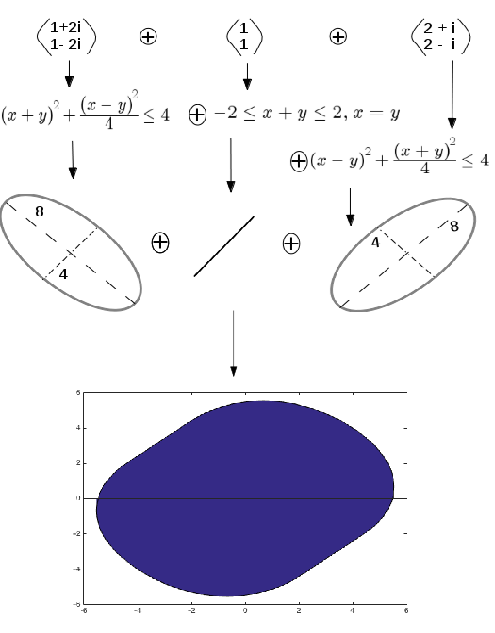
\includegraphics[scale=0.43]{fig/cznew.png}\\[1em]
%% 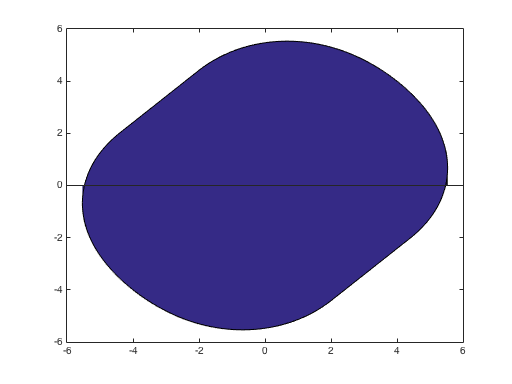
\includegraphics[scale=0.5]{fig/CZhull.png}
%% \caption{Real projection of a complex zonotope as\\ Minkowski sum of 2 ellipses and 1 line segment }~\label{fig:cz}
%% \end{figure}
%% %

As the real projection of the generator of a complex zonotope can
either be an ellipsoid or a line segment, a complex zonotope can
represent a Minkowski sum of line segments as well as some
ellipsoids.  The non-polyhedral real projections along the three axis
oriented hyperplanes of the following 3-D complex zonotope is shown in
Figure~\ref{fig:3dcztope}
%
\[
\cztope{\mymatrix{-0.2226  & -0.1335 + 0.1769\iota  & -0.1335 - 0.1769\iota\\
   0.3615 &   0.2713 + 0.3991\iota &  0.2713 - 0.3991\iota\\
   0.2446 &  -0.8473 &  -0.8473}}{0}
\]
%
\begin{figure}
\center
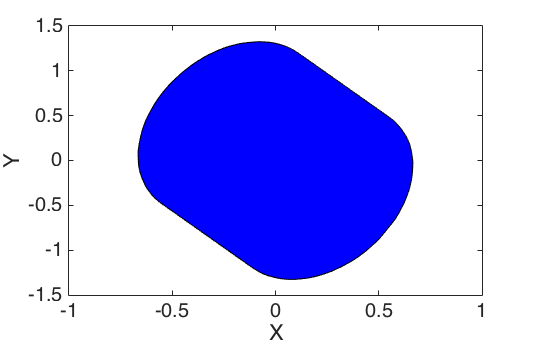
\includegraphics[scale=0.5]{fig/CZtopes/xycz.png}
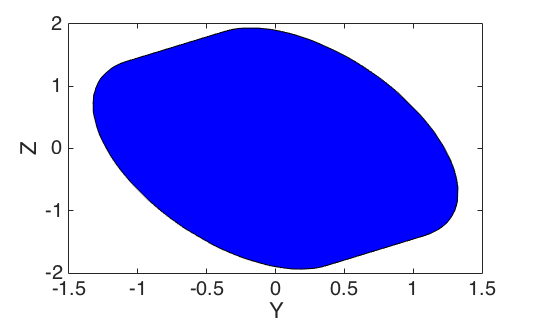
\includegraphics[scale=0.5]{fig/CZtopes/yzcz.png}
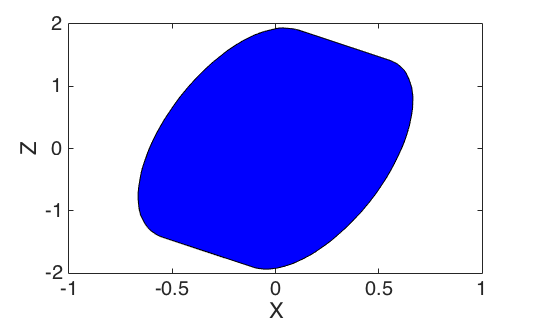
\includegraphics[scale=0.5]{fig/CZtopes/xzcz.png}
\caption{Real projection of complex zonotope on axis oriented hyperplanes}~\label{fig:3dcztope}
\end{figure}
%

\emph{Contraction along eigenvectors:  }  A motivation for extending
simple zonotopes to complex zonotopes is that a complex zonotope with
its generators as the complex eigenvectors of a discrete time linear
system is positively invariant if the complex eigenvalues
corresponding to the generators are bounded within unity in their
absolute values.  This is because the generators of the resultant
complex zonotope after transformation will be scaled by the absolute
values of the corresponding eigenvalues.  For example, consider the
following matrix $A$ and the complex zonotope
$\cztope{V}{0}$ generated by the complex eigenvectors of $A$.
%
\begin{align*}
& A=\mymatrix{
0.1502 &  -0.0438  &  0.1366\\
    0.7482 &   0.1470  &  0.1251\\
   -0.8436 &  -0.7027  &  0.0418
}\\
& V=\mymatrix{
-0.2226  &  -0.1335 + 0.1769\iota &  -0.1335 - 0.1769\iota\\
   0.3615 &   0.2713 + 0.3991\iota &  0.2713 - 0.3991\iota\\
   0.2446 & -0.8473 &   -0.8473 
}
\end{align*}
%
The eigenvalues of $A$ are $-0.2291$, $0.1339 + 0.5071\iota$ and
${0.1339 - 0.5071\iota}$, whose absolute values are $0.2291$,
$0.5245$, and $0.5245$, respectively.  After the transformation by
$A$, the set generated by $V^T_1$ gets scaled down to $0.2291$ times
its size and that of $V^T_2$ and $V^T_3$ to $0.5245$ times
its their size.  So, the complex zonotope, which is a Minkowski sum
of these sets, contracts after the transformation.  This is illustrated
in Figure~\ref{fig:cz-scaled-down}, which shows the contraction of
each of the sets formed by the generators and the consequent
contraction of the complex zonotope.
%
\begin{figure}
\center
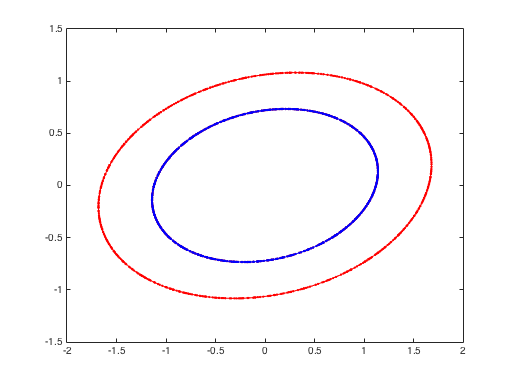
\includegraphics[scale=0.4]{fig/CZtopes/eigcontraction.png}
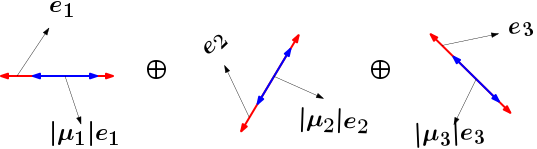
\includegraphics[scale=0.5]{fig/CZtopes/contraction-zonotope.png}
\caption{Contraction of complex zonotope along
eigenvectors}~\label{fig:cz-scaled-down}
\end{figure}
%
This property of contraction of complex zonotope by a linear
transformation based on the eigenstructure of a matrix is explained
mathematically in the following proposition.
%
\begin{proposition}[Eigenstructure based invariance]~\label{lem:eig-invariance}
Let us consider $\ptemp\in\mat{n}{n}{\compnums}$ consists of the
complex eigenvectors of a matrix $A\in\mat{n}{n}{\reals}$ as its
column vectors and $\mu\in\compnums^n$ be the vector of complex
eigenvalues, i.e., $A\ptemp = \ptemp\diagonal{\mu}$.
Then \[A\lt(\cztope{\ptemp}{0}\rt)
= \cztope{\ptemp\diagonal{{\mu}}}{0}.\]  If
$\infnorm{\mu}\leq 1$, then
$A\lt(\rztope{\ptemp}{0}\rt)\subseteq \rztope{\ptemp}{0}$.
\end{proposition}
% 
\begin{proof}
We derive
  %
\begin{align*}
& A\lt(\cztope{\ptemp}{0}\rt) =
A\set{\ptemp\zeta:~\zeta\in\compnums^n,\infnorm{\zeta}\leq 1}\\
& =\set{A\ptemp\zeta:~\zeta\in\compnums^n,\infnorm{\zeta}\leq 1}
= \cztope{A\ptemp}{0}=\cztope{\ptemp\diagonal{\mu}}{0}.
\end{align*}
%
which proves the first part of the
Proposition.

For the second part, we are given that $\infnorm{\mu}\leq 1$.
Consider a point
%
\begin{align*}
  & y\in A\cztope{\ptemp}{0}=\cztope{\ptemp\diagonal{\mu}}{0}~~\text{where}\\
  &y = \ptemp\diagonal{\mu}\delta:\infnorm{\delta}\leq
1.
\end{align*}
%
Let $\zeta = \diagonal{\mu}\delta$. Then $\infnorm{\zeta} \leq
\infnorm{\mu}\infnorm{\delta} \leq 1$.  So,
%
\begin{align*}
  & y=\ptemp\zeta~~\text{ where }~
  \infnorm{\zeta}\leq 1.
\end{align*}
%
So, we get $y\in \cztope{\ptemp}{0}$.  As this is true for all
$y\in\cztope{\ptemp}{0}$, we have
$A\lt(\cztope{\ptemp}{0}\rt)\subseteq
\cztope{\ptemp}{0}$ when $\infnorm{\mu}\leq 1$.
\end{proof}
%If we add more generators to the above representation of a complex
zonotope, it would increase the size of the complex zonotope.
Therefore, we can not find better approximations of a given set by
only adding more generators to the complex zonotope.  Moreover, adding
a generator can violate positive invariance.  For example, consider
the complex zonotope $\cztope{\ptemp}{0}$, where
%
\[
\ptemp = \mymatrix{-0.2226 &  -0.1335 + 0.1769\iota &   -0.1335 - 0.1769\iota\\
   0.3615  &   0.2713 + 0.3991\iota &   0.2713 - 0.3991\iota\\
   0.2446  &   -0.8473 &  -0.8473}.
\]
%
The above complex zonotope contracts after transformation by the matrix
%
\[
A = \mymatrix{-0.2766 &   -0.0806 &    0.2516\\
    1.3779  &  0.2707  &   0.2304\\
   -1.5536 &  -1.2942 &    0.0769}
\]
%
as shown in Figure~\ref{fig:refinement}.  On the other hand, when we
add another generator $\mymatrix{0 & 0.5 & 0.5}^T$, then the complex
zonotope, $\cztope{W}{0}$, where
%
\[
W=\mymatrix{-0.2226 &  -0.1335 + 0.1769\iota &   -0.1335 -
   0.1769\iota & 0\\
   0.3615 &   0.2713 + 0.3991\iota &   0.2713 -
   0.3991\iota & 0.5\\
   0.2446 &   -0.8473 + 0.0000\iota &  -0.8473 & 0.5}
\]
%
does not contract as illustrated in Figure~\ref{fig:refinement}.
%
\begin{figure}
\center
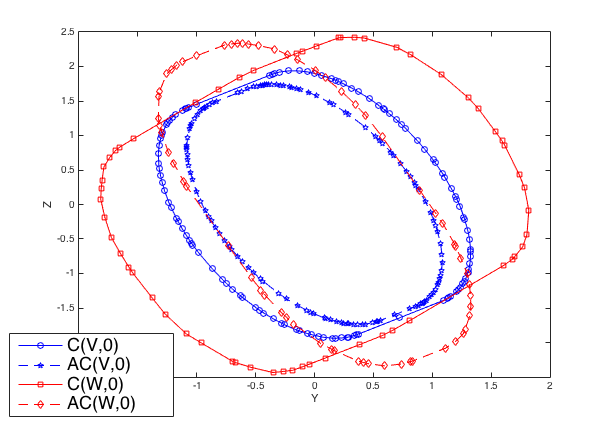
\includegraphics[scale=0.5]{fig/CZtopes/refinement.png}
\caption{Violation of positive invariance and size increase after
adding a generator to the basic representation.}~\label{fig:refinement}
\end{figure}

Alternatively, to refine
a complex zonotope, we can adjust the magnitude of contribution of
each generator to the size of the set while also preserving the
positive invariance.  This way, can also add more generators and
increase approximation accuracy by adjusting the magnitudes of each
generator.  In order to conveniently perform algebraic manipulations
on the magnitude of each generator, we can explicitly specify variable
bounds on the combining coefficients.  This gives us a more general
representation, which we call as {\it template complex zonotope},
where the magnitude of each combining coefficient is bounded in its
absolute value a {\it scaling factor}.  We call the matrix whose
column vectors generate a template complex zonotope as a {\it
template}.  This representation is similar in spirit to the known
template based set
representations~\cite{Sankaranarayanan+Dang+Ivancic-08-Symbolic,DBLP:journals/lisp/Mine06}
in abstract interpretation, where for some fixed template, subsets of
metric spaces are mapped to points in a lattice.  In the case of a
template complex zonotope, for a fixed template, subsets of the
complex vector space can be mapped to the {\it scaling factors}.
%
\begin{definition}[Template complex zonotope]
Let us consider ${\ptemp\in\mat{n}{m}{\compnums}}$ called the template,
${\sfact\in\reals^m_{\geq 0}}$ called scaling factors and
${\cen\in\compnums^n}$ called the center.  Then the following is a template
complex zonotope.
%
\begin{equation}
\tcztope{\ptemp}{\cen}{\sfact}
= \set{\ptemp\zeta+\cen:~\absolute{\zeta_i}\leq \sfact_i~\forall
i\in\set{1,...,m}}.
\end{equation}
\end{definition}
In further discussion, we use the term {\it representation size} of a
template complex zonotope to refer to the size of the template matrix.
In the rest of this chapter, we consider the following notation,
unless otherwise specified.
%
\[
\ptemp\in\mat{n}{m}{\compnums},~~\cen\in\compnums^n,~~\sfact\in\reals^m_{\geq 0}.
\]
%
A template complex zonotope can be converted to the basic
representation of the complex zonotope by multiplying the diagonal
matrix of scaling factors to the template.  This is described in the
following lemma.
%
\begin{lemma}[Normalization]~\label{lem:normalization}
Let us consider ${\mu\in\compnums^m}$.
%
\begin{align*}
\text{Then}\hspace{3em}&\tcztope{\ptemp\diagonal{\mu}}{\cen}{\sfact}=\tcztope{\ptemp}{\cen}{\diagonal{\absolute{\mu}}\sfact}.~\numberthis\label{eqn:normalization}\\
\text{Therefore},\hspace{3em} & \tcztope{\ptemp}{\cen}{\sfact}=\cztope{\ptemp\diagonal{\sfact}}{\cen}.
\end{align*}
%
\end{lemma}
%
\begin{proof}
Consider a point $x\in\tcztope{\ptemp\diagonal{\mu}}{\cen}{\sfact}$,
where
%
\[
x=\cen+\ptemp\diagonal{\mu}\zeta:\absolute{\zeta}\leq\sfact.
\]
%
Let $\zeta^\pr=\diagonal{\mu}\zeta$.  Then, $x=c+\ptemp\zeta^\pr$.
We get
%
\[
\absolute{\zeta^\pr}=\diagonal{\absolute{\mu}}\absolute{\zeta}\leq\diagonal{\absolute{\mu}}\sfact.
\]

Therefore, ${x\in\tcztope{\ptemp}{\cen}{\diagonal{\mu}\sfact}}$.  This
means,
%
\[
\tcztope{\ptemp\diagonal{\mu}}{\cen}{\sfact}\subseteq\tcztope{\ptemp}{\cen}{\diagonal{\absolute{\mu}}\sfact}
\]
%
Next consider a point
$y\in\tcztope{\ptemp}{\cen}{\diagonal{\absolute{\mu}\sfact}}$ where
%
\[
y=\cen+\ptemp\epsilon:~\absolute{\epsilon}\leq
\diagonal{\absolute{\mu}}\sfact.
\]
%
Let us consider $\epsilon^\pr\in\compnums^m$, such that
%
\[\forall i\in\set{1,...,m},~~
\epsilon_i=\left\{
\begin{array}{l}
\frac{\epsilon_i}{\mu_i}~\text{if}~\mu_i\neq 0\\
0~\text{if}~\mu_i=0.
\end{array}
\right.
\]
%
We shall show that $\epsilon=\epsilon^\pr\diagonal{\mu}$, i.e., for
any $i\in\set{1,...,m}$, $\epsilon_i=\epsilon^\pr_i\mu_i$.  We prove
it in the following two cases.
\begin{enumerate}
\item Let us consider $\epsilon_i\neq 0$.  As
$\absolute{\epsilon}\leq\absolute{\diagonal{\mu_i}}\sfact$, so
  $\mu_i\neq 0$.  Therefore,
  \[
  \epsilon_i=\frac{\epsilon_i}{\mu_i}\mu_i=\epsilon^\pr_i\mu_i.
  \]
\item Let us consider $\epsilon_i=0$.  As
$\absolute{\epsilon}\leq\absolute{\diagonal{\mu_i}}\sfact$, so $\mu_i=
  0$.  This implies
  \[
  0=\epsilon=\epsilon^\pr_i\times
  0=\epsilon^\pr_i\mu_i.
  \]
  %
\end{enumerate}
%
So, we get $y=\cen+\ptemp\diagonal{\mu_i}\epsilon^\pr$.  By the definition of
$\epsilon^\pr$, we get
%
\[\forall i\in\set{1,...,m}~~
\absolute{\epsilon^\pr_i}\leq
\left\{
\begin{array}{l}
\absolute{\frac{\epsilon_i}{\mu_i}}\leq\frac{\absolute{\mu_i}\sfact_i}{\absolute{\mu_i}}=\sfact_i~\text{if}~\mu_i\neq
0\\
0~\text{if}~\mu_i=0
\end{array}
\right.
\]
%
Therefore, $\absolute{\epsilon^\pr}\leq\sfact$.  So,
$y\in\tcztope{\ptemp\diagonal{\mu}}{\cen}{\sfact}$.  Therefore,
%
\[
\tcztope{\ptemp}{\cen}{\diagonal{\absolute{\mu}}\sfact}\subseteq\tcztope{\ptemp\diagonal{\mu}}{\cen}{\sfact}.
\]
%
Combining the previous two conclusions, we get
Equation~\ref{eqn:normalization}.

By definition,
%
\begin{align*}
& \cztope{\ptemp\diagonal{\sfact}}{\cen}=\tcztope{\ptemp\diagonal{\sfact}}{\cen}{\repmat{1}{m}{1}}\\
& \%\%~~\text{by Equation~\ref{eqn:normalization}}\\
& =\tcztope{\ptemp}{\cen}{\diagonal{{\sfact}}\repmat{1}{m}{1}}=\tcz{\ptemp}{\cen}{\sfact}.~\hspace{3em}\qedhere
\end{align*}
%
\end{proof}
%
